\documentclass[10pt]{article}
\usepackage[utf8]{inputenc}
\usepackage{listings}
\usepackage{float}
\usepackage{graphicx}
\usepackage{fullpage}
\usepackage{caption}
\usepackage{subcaption}
\usepackage{amsmath}
\usepackage{hyperref}

%\renewcommand{\thesubsection}{\arabic{subsection}}
\renewcommand{\thesubsubsection}{\alph{subsubsection}}

\title{Pattern Recognition Practical 4}
\author{Group 24: \and Maikel Withagen (s1867733) \and Steven Bosch (s1861948)}
\date{\today}
\lstset{
frame=single, 
numbers=left, 
breaklines=true, 
language=Matlab,
basicstyle=\small, 
title=\lstname
}

\renewcommand{\thesection}{Assignment \arabic{section}}
\renewcommand{\thesubsection}{\arabic{subsection}}
\begin{document}
\section{Assignment 1}
\subsection{}
Using the code given in the appendix we created the scatterplot in figure \ref{fig1.1}.

\begin{figure}[H]
 \centering
 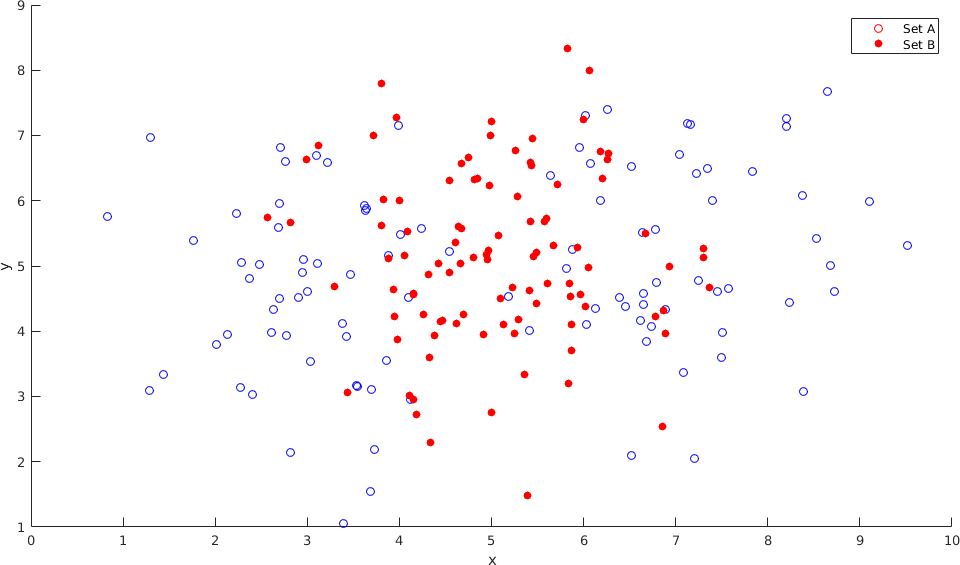
\includegraphics[width=\textwidth]{Fig1_1.png}
 \caption{Scatterplot for the two classes.}
 \label{fig1.1}
\end{figure}

The plot shows that there are at least three prototypes needed to approach a fairly well classification of these data. Two for set A, which should probably be located around $(3,4.5)$ and $(7.5, 5.5)$, and one for set B somewhere around $(5,5)$. 

\subsection{}
The code in the appendix shows our implementation of the LVQ1 algorithm. We acquired the following results for the different settings.

\subsubsection{1 Prototype for class A and 1 prototype for class B}

\begin{figure}[H]
 \centering
 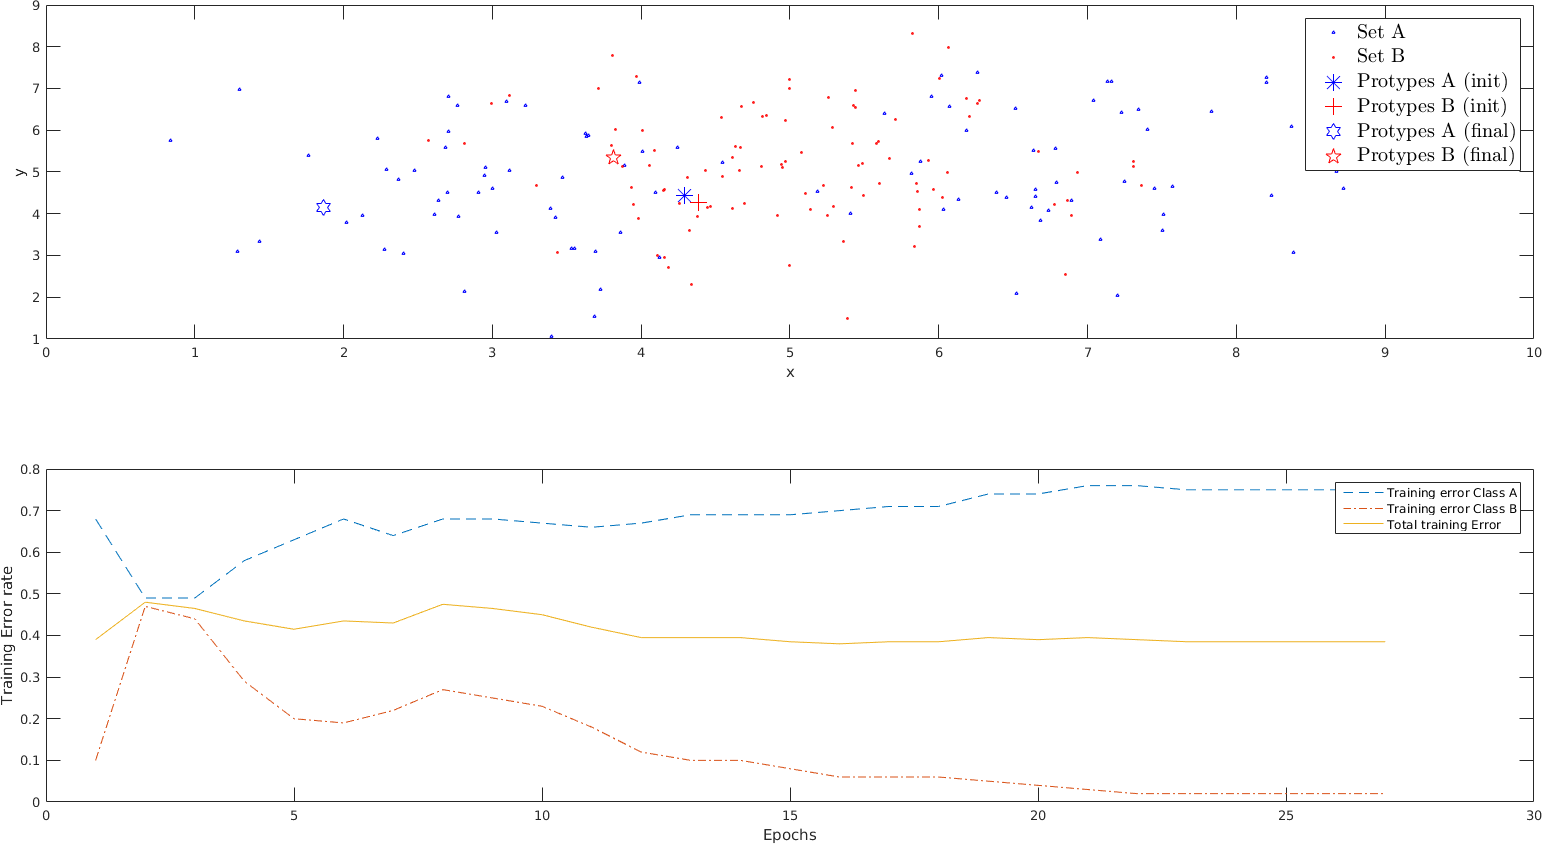
\includegraphics[width=\textwidth]{Fig12_a1.png}
 \caption{Classification for 1 prototype for class A and 1 prototype for class B. Plot two gives the corresponding error rates (Class 1 is A and class 2 is B).}
 \label{fig1.12a}
\end{figure}
As is expected with only one prototype per class, figure \ref{fig1.12a} shows that the prototype for class B is formed quite well, allowing it to correctly classify at least the data points that belong to class B (an error stabilising at around 0.05). However, since class A is distributed in two groups, with B in between them, the prototype for class A is formed in the center of one of the two outer clusters, which means it can only correctly classify that cluster correctly. The other cluster will be incorrectly classified as class B, which follows from the error rate which stabilises at around 0.38, meaning that on average 38 out of 100 data points are incorrectly classified, which is quite high.

\subsubsection{1 Prototype for class A and 2 prototype for class B}

\begin{figure}[H]
 \centering
 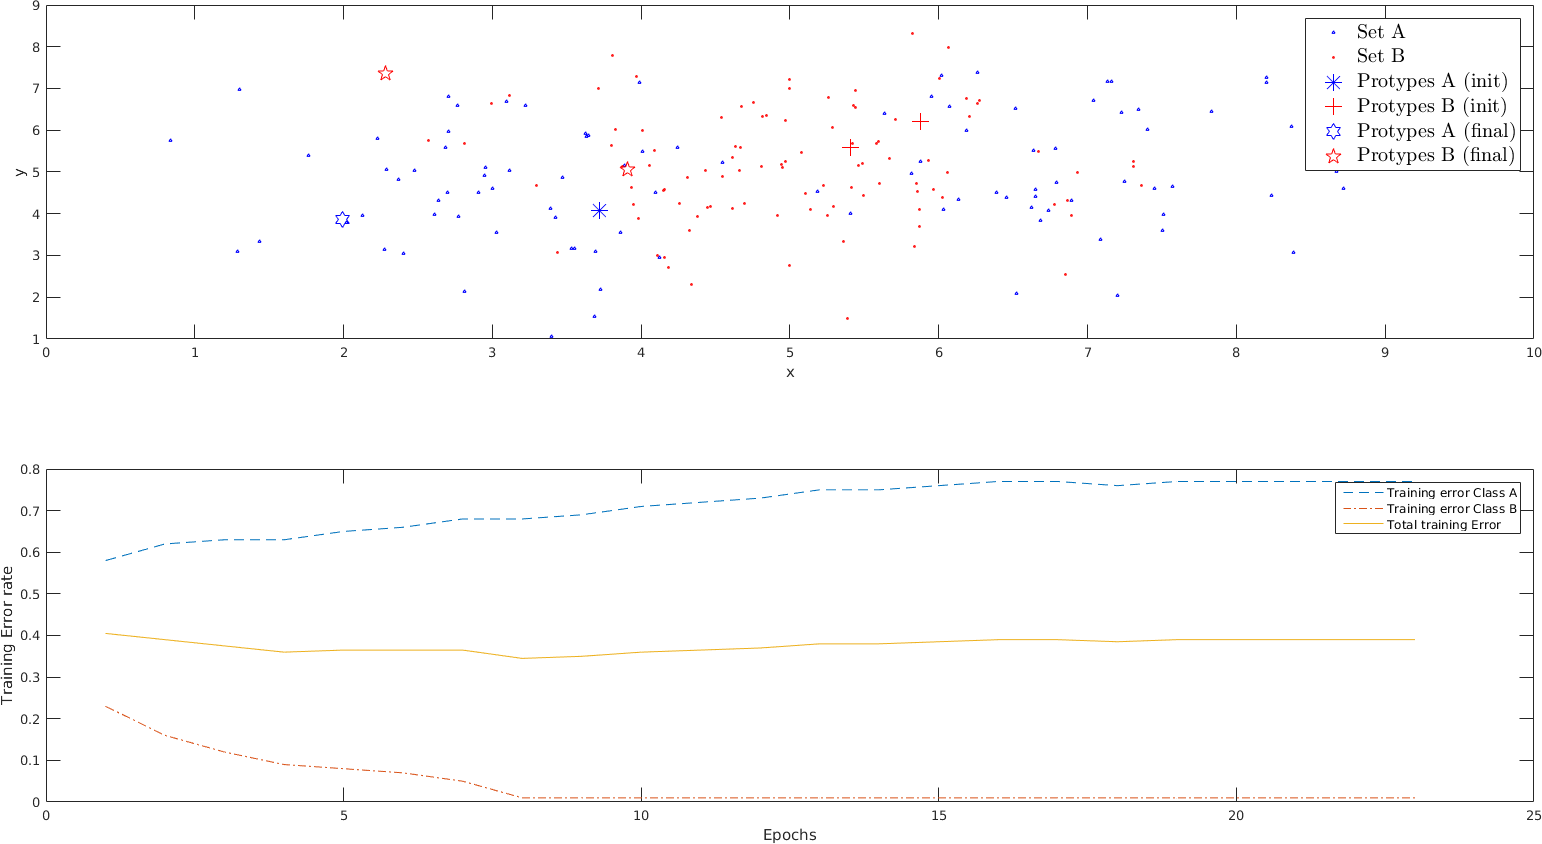
\includegraphics[width=\textwidth]{Fig12_b.png}
 \caption{Classification for 1 prototype for class A and 2 prototypes for class B. Plot two gives the corresponding error rates (Class 1 is A and class 2 is B).}
 \label{fig1.12b}
\end{figure}
In this case figure \ref{fig1.12b} shows the same thing happening with the prototype for class A: it ends up in one of the two separated A-clusters. Its error is therefore also similar to that in the previous case. On the other hand we see that the two prototypes for class B, even though the data points belonging to class B are clustered in one big cluster, we see that a second prototype slightly improves the result, giving an error that stabilises near 0. This might be the case because it `catches' some of the last data points that were mixed in with the left-side class A cluster, meaning that it also causes some of the class-B data points in that cluster to be misclassified. This explains the fact that the error of class A has become slightly higher, resulting in a total error that is approximately the same as in the previous case.

\subsubsection{2 Prototype for class A and 1 prototype for class B}

\begin{figure}[H]
 \centering
 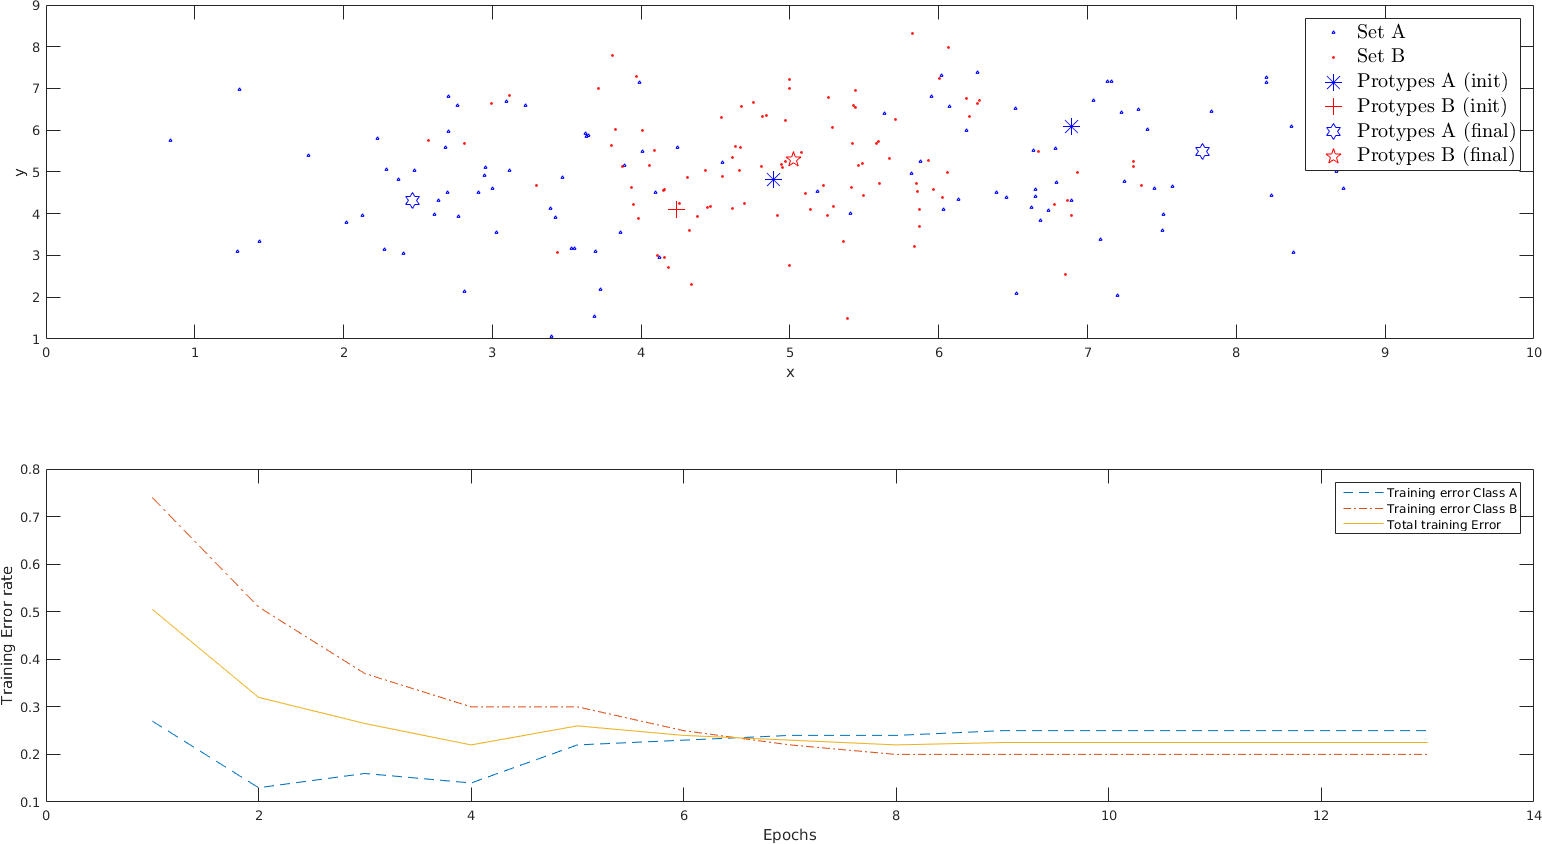
\includegraphics[width=\textwidth]{Fig12_c.png}
 \caption{Classification for 2 prototypes for class A and 1 prototype for class B. Plot two gives the corresponding error rates (Class 1 is A and class 2 is B).}
 \label{fig1.12c}
\end{figure}
In this case figure \ref{fig1.12c} shows a much lower error rate than in the previous two cases. This is due to the fact that there are now two prototypes for class A, which can classify the seperated data points much better, since they are grouped into two clusters (one prototype for the left cluster, one for the right). Ultimately this results in a total error that stabilises around 0.22, which is significantly lower than in the previous two cases.

\subsubsection{2 Prototype for class A and 2 prototype for class B}

\begin{figure}[H]
 \centering
 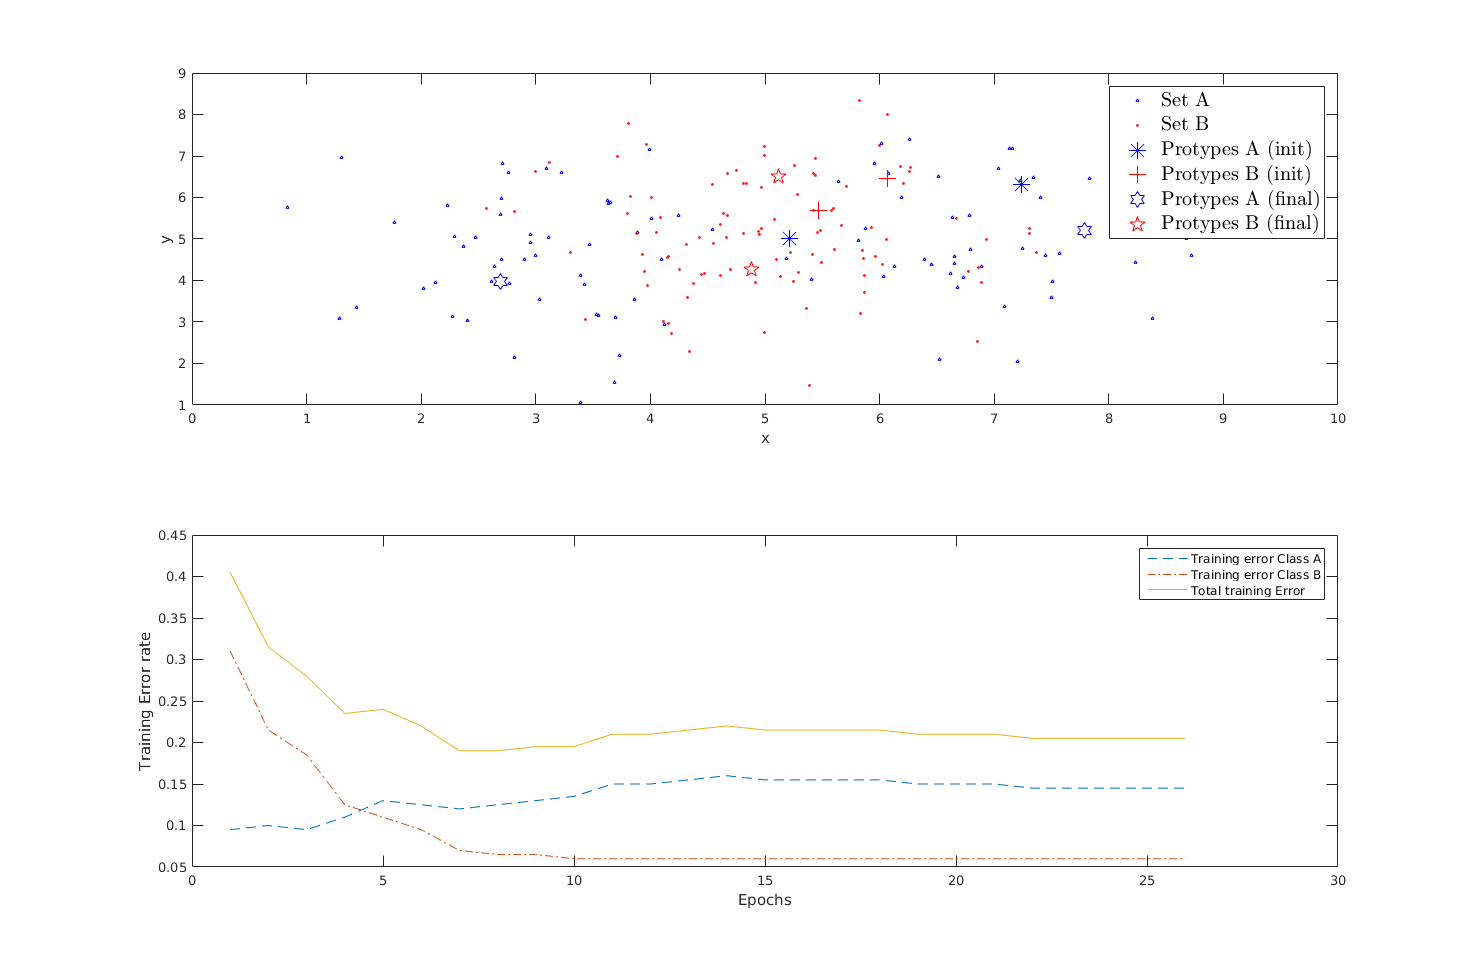
\includegraphics[width=\textwidth]{Fig12_d.png}
 \caption{Classification for 2 prototypes for class A and 2 prototypes for class B. Plot two gives the corresponding error rates (Class 1 is A and class 2 is B).}
 \label{fig1.12d}
\end{figure}
Finally in the case of two prototypes for each class, figure \ref{fig1.12d} shows slightly worse results than for the previous case, with a total error stabilising at approximately 0.23. This has probably to do with the two prototypes for class B now being divided over the one cluster of data points, which causes them to be slightly nearer to the data points that belong to class A. This causes some of those data points to be misclassified, resulting in a slightly higher error.

\bigskip
\noindent Overall we can state that the case for two prototypes for class A and one for class B yields the best results for this particular data set. This is of course also the intuitve explanation, since any human can immediately see that the clusters are distributed in such a way that this distribution of prototypes is needed.


\section*{Appendix}
\lstinputlisting{../Code/Ass1_1.m}
\lstinputlisting{../Code/Ass1_2.m}


\maketitle
\end{document}
